\documentclass[a4paper, 10pt, titlepage]{report}
\usepackage[utf8]{inputenc}
\usepackage[english, vietnamese]{babel}
\usepackage{authblk}
\usepackage{setspace}
\usepackage[margin=1in, a4paper]{geometry}
\usepackage{graphicx}
\graphicspath{ {./figures/} }
\usepackage{subcaption}
\usepackage{amsmath}
% \usepackage{lineno}
\usepackage[hidelinks]{hyperref}
\usepackage{mlmodern}
\usepackage{svg}
% \linenumbers
\selectlanguage{english}
%%%%%% Bibliography %%%%%%
% Replace "sample" in the \addbibresource line below with the name of your .bib file.
\usepackage[style=nejm, 
citestyle=numeric-comp,
sorting=none]{biblatex}
\usepackage{listings}
\lstset{
basicstyle=\small\ttfamily,
columns=flexible,
breaklines=true
}
% \addbibresource{sample.bib}

%%%%%% Title %%%%%%
% Full titles can be a maximum of 100 characters, including spaces. Do not use abbreviations.
% Title Format: Use title case, capitalizing the first letter of each word, except for certain small words, such as articles and short prepositions
\title{Chess Game Project}

%%%%%% Authors %%%%%%
% Authors should be listed in order of contribution to the paper, by first name, then middle initial (if any), followed by last name.
% Authors should be listed in the order in which they will appear in the published version if the manuscript is accepted. 
% Use an asterisk (*) to identify the corresponding author, and be sure to include that person’s e-mail address. Use symbols (in this order: †, ‡, §, ||, ¶, #, ††, ‡‡, etc.) for author notes, such as present addresses, “These authors contributed equally to this work” notations, and similar information.
\begin{otherlanguage}{vietnam}
\author{Nguyễn Hoàng Thuận Phát, Huỳnh Tấn Phúc}    
\date{Submission day: \selectlanguage{english}\today}
\end{otherlanguage}
%%%%%% Affiliations %%%%%%

%%%%%% Date %%%%%%
% Date is optional
% \date{}

%%%%%% Spacing %%%%%%
% Use paragraph spacing of 1.5 or 2 (for double spacing, use command \doublespacing)
\onehalfspacing

\begin{document}

\maketitle
\selectlanguage{english}
\renewcommand{\abstractname}{Overview}
%%%%%% Abstract %%%%%%
\begin{abstract}
  The project aims to develop a chess game that is smooth, minimalistic, lightweight in size and performance while providing decent experience to player.
\end{abstract}

%%%%%% Main Text %%%%%%
%A few notes on the main text:  
%Three heading levels are permitted. Only the headings listed are permitted as Level 1 headings. Authors are encouraged to indicate the level of each heading using a unique format. For example, 
%\textbf{LEVEL 1 IN BOLD CAPS}
%\textbf{Level 2 in bold}
%\textit{Level 3 in italics}
% \pagebreak
\tableofcontents
\chapter{Requirement}

%%%%% Citations in the text %%%%%%
\section{Game modes}
\begin{itemize}
  \item 2-player mode
        \begin{itemize}
          \item 2 players can play against each other on the same instance
          \item Player's turn is managed automatically, alternating between player 1 (white) and player 2 (black)
        \end{itemize}
  \item Versus AI mode: Player as white pieces plays against black pieces controlled by Stockfish chess engine, with three level of difficulty
        \begin{itemize}
          \item Easy mode: Stockfish is ran with high variation and low evaluation level. It searches for next move to depth 1 in 100 milisecods, and has limited computing resource.
          \item Medium mode: Stockfish is ran with moderate variation and moderate evaluation level.Stockfish searches for next move to depth 3 in 400 miliseconds and more computing resource are allocated
          \item Hard mode. Stockfish are given the most computing resource. It plays perfectly without variation, searches to depth 20 in 2000 miliseconds
        \end{itemize}
        AI's turn is delayed for 500 miliseconds in addition to Stockfish's search time to avoid runtime errors.
\end{itemize}
%%%%%% Equations %%%%%%

\section{User Interface(UI)}
\begin{itemize}
  \item A chessboard with movable pieces

  \item A start menu that renders before a game is started
        \begin{itemize}
          \item Start buttons that start the game in two-player mode and single player mode. If the game is started in single player mode, there is a popup menu for the user to select the difficulty of AI.
          \item Load button to load saved board states from storage.
          \item Quit button to exit the game.
        \end{itemize}
  \item An in-game menu is rendered to the right and bottom portions of the board.
        \begin{itemize}
          \item Promotion menu is rendered to the top or bottom of pawn under promotion, with four options to promote to queen, bishop, kngiht or rook.
          \item Right menu bar

                \begin{itemize}
                  \item Button to save and load current board configuration, including board state, game mode and AI diffculty if there is.
                  \item Button to access setting menu
                \end{itemize}

          \item Bottom menu bar
                \begin{itemize}
                  \item Button to undo the latest move and undo to the initial board state.
                  \item Button to redo the latest undo and redo to the latest board state.
                \end{itemize}
        \end{itemize}
  \item A load menu displays buttons to load saved games, each of which shows previews of board when hovered and load the actual game when clicked.
  \item A save menu displays buttons to save current game. On hover, each button display preview of saved game that is going to be overwritten if current game is saved. When pressed, a confirmation menu appears to ask if user want to overwrite. There are also a clear button for each save file to delete that save.
  \item A setting menu has buttons of switching theme along with the theme's designated pieces set, adjust volume of all sound effect, mute and unmute sound, reset the game to starting position, and quit to menu.
\end{itemize}
\section{Chess board representation}
\begin{itemize}
  \item Chessboard is drawn using SDL2 graphic libraries.
  \item Pieces are first parsed to bitmap using \href{https://github.com/memononen/nanosvg}{nanoSVG} library's function, then rasterized and rendered by SDL2's functions.
  \item Pieces are moved by drag-dropping with mouse.
  \item Legal moves are highlighted with cell-centered dots for moves and hollow circles for captures. The rendering of legal moves are triggered when player click on a piece or drop a piece to its original cell.
  \item Illegal moves (including movement to cells that are not highlighted, movement out of board's bound, etc) will return the piece to its original cell and does not count as a move.
  \item Moves are managed automatically, alternating between two colors after each move. Current player's turn is displayed by an indicator on the top portion of the screen.
  \item King piece's cell is highlighted with different colors for its check, checkmate and stalemate statuses.
        \begin{itemize}
          \item To highlight chess piece's movement, color of initial and ending cells of that piece is mixed with a yellowish color.
          \item To highlight check status of king piece, color of its cell is mixed with a redish color.
          \item To highlight checkmate status of king piece, color of its cell is replaced with a bright red color.
          \item To highlight stalemate status of king piece, color of its cell is mixed with a cyan color.
        \end{itemize}
\end{itemize}
\section{Game Logic}
\begin{itemize}
  \item Pieces' movement
        \begin{itemize}
          \item Chess pieces' moves are generated on selection based on their position, then get processed to create list of moves and capture in each direction.
          \item Special moves' condition are reviewed after each move, based on their condition they will get added to suitable pieces in the next move.
          \item Status of king is examined during moves generating and after all special moves.
        \end{itemize}
  \item Selected cell's ending cell is compared in its legal moves and captures list. Each move is simulated while creating the list to ensure that move does not put the king in check.
  \item In case of stalemate or checkmate, any chess piece cannot be moved. In such case, a pop-up menu is displayed to ask if user want to continue another game. If yes button is clicked, the game reset to starting configration with the current game mode. If no button is clicked, the game quits. If the menu is turned off, the game still function as normal, yet the board cannot be interacted with.
\end{itemize}
\section{AI Opponent}
Stockfish is initialized before running with
\begin{verbatim}
uci
setoption name Hash value 128
setoption name Threads value 1
isready
\end{verbatim}

For each time the game is started from new board or from save file, command \texttt{ucinewgame} is sent to Stockfish

There are three modes of AI opponent lining up with three difficulty: Easy, Medium and Hard.
\begin{itemize}
  \item Easy difficulty: Stockfish is configured with \begin{verbatim}
setoption name Skill level value 0
setoption name Threads value 1     
setoption name Hash value 16      
setoption name MultiPV value 10    
\end{verbatim} and execute \texttt{go depth 2 movetime 300} after setting FEN notation for board state.
  \item Medium difficulty: Stockfish is configured with \begin{verbatim}
setoption name Skill level value 3
setoption name Threads value 2     
setoption name Hash value 64      
setoption name MultiPV value 5    
\end{verbatim} and execute \texttt{go depth 3 movetime 400} after setting FEN notation for board state.
  \item Hard difficulty: Stockfish is configured with \begin{verbatim}
setoption name Skill level value 20
setoption name Threads value 8     
setoption name Hash value 2048      
setoption name MultiPV value 1    
\end{verbatim} and execute \texttt{go depth 20 movetime 2000} after setting FEN notation for board state.
\end{itemize}
After letting Stockfish executing commands, the communicator wait for 500 miliseconds before reading the result from \texttt{tmp/stockfish\_output.txt}
\section{Game state management}
The game is managed using the combination of 2D array board representation and FEN notation, the latter stores information needed to reconstruct the board from scratch. Turn management is done right after a legal move had been made. After each legal move, both array representation and FEN notation of the board is updated.

For undo and redo features, two stacks of FEN notation is used to store information for those operation, with the top of undo stack is the current board state. FEN notation of initial state is also saved as a constant string for creation of new game.

\section{Save and Load Functionality}
\subsection{Save}
There is separate menu dedicated for saving. In that menu, available save files are displayed in cards on the left side. On hovering, the card being hovered will be highlighted, and the board state that is stored within the file that the card stand for is displayed to the right of the game windows. When user clicks on a card, the confirmation box appears, asking if user want to overwrite the save file. If the user confirms, the game will proceed to overwrite that save file, otherwise the confirmation box will close.
\subsection{Load}
There is separate menu dedicated for loading. In that menu, available save files are displayed in cards on the left side. On hovering, the card being hovered will be highlighted, and the board state that is stored within the file that the card stand for is displayed to the right of the game windows as a preview. When user clicks on a card, the board immediately load the respective save file.
\section{Optional features}
While being dragged, selected chess piece follows the mouse's cursor smoothly.
\section{Technology stack}
The game's logic, game state management and GUI(graphic user interface) is written in C and C++, using SDL2 and nanoSVG libraries for graphic. The AI used for player versus computer mode is \href{https://github.com/official-stockfish/Stockfish}{Stockfish}, a popular and strong open-source AI chess engine. Current board state is written to plain text file in FEN notation, followed by numbers indicating current game mode and difficulty of AI opponent.
\chapter{Design document}
\section{System requirement and build}
Currently, the game is only developed and tested on Windows operating system.
To compile the program from source files, the directory must first be at the same path as the makefile file, that is, the \texttt{CS160\_Chess} folder. Also, makefile must be installed.

Then, user can build the project by running \texttt{./buildscriptwindows.ps1} or run \texttt{make all}. After that, the executable is named \texttt{chess.exe}, which is located at \texttt{CS160\_Chess} folder. The executable will be automatically be ran after being built.

An alternative way for building the project if the above methods doesn't work is to run \\ \texttt{BuildScriptWindows.ps1} file in powershell. 

\section{Architecture design}
\includesvg[width = 500pt, height = 600pt, angle = 0]{altDecision.svg}

\section{Processes}
\subsection{Player's move}
\includegraphics[width = \linewidth]{MOve diagram.png}
\subsection{AI's move}
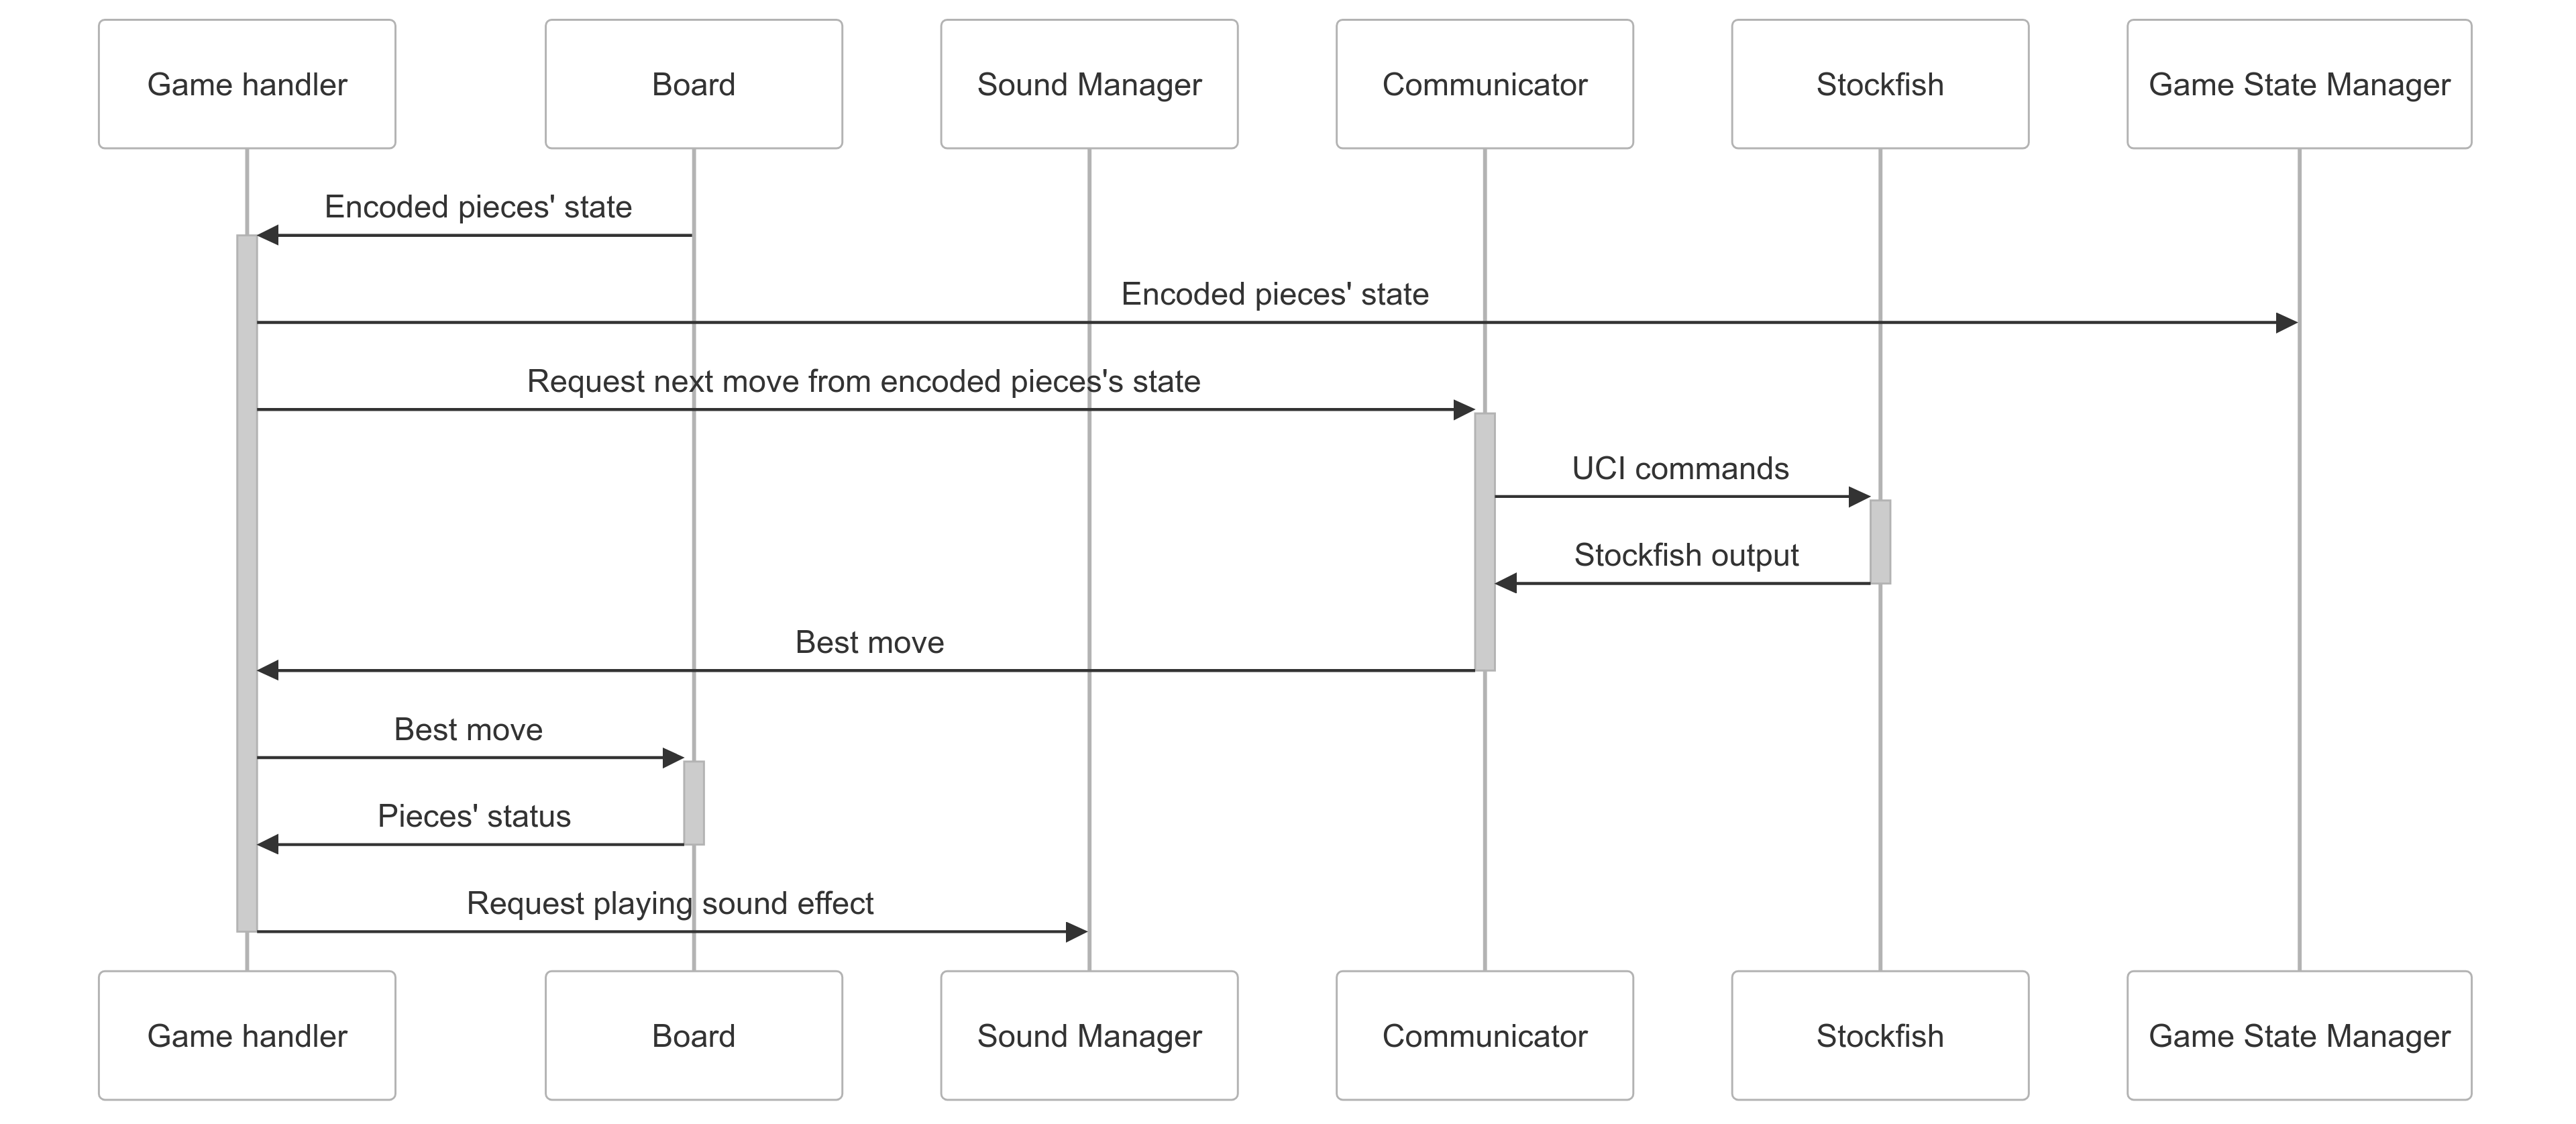
\includegraphics[width = \linewidth]{AI move.png}
\section{User Interface}
\subsection{Consistent Color theme}
The game adopts the subtle green and beige color gradient, which was taken inspiration from a famous online Chess game website \href{https://chess.com/}{Chess.com}.

The gradient is applied to UI elements like Chess board, Turn indicator, Buttons and menus. Different Themes also are provided for player to choose from.

The game aims to support extended play sessions and reduce eye strain by implementing a dark mode with muted Gray and Green asthetic.
\subsection{Clarity and Simplicity}
The game utilizes clean, flat design elements that align with the Windows 11 Fluent Design language to ensure a modern and accessible look.

Prioritize clear visibility of the board and pieces. Use distinct, high-contrast color pallete to enhance focus.

Visual distractions are limitedby avoiding excessive animations or decorative elements that do not serve gameplay.
\subsection{Minimalism in Navigation}
The game implements an intuitive and minimal navigation bar with essential options (e.g., Play, Load, Settings). Avoid clutter by grouping advanced features under expandable menus.

Keep action buttons (e.g., "Undo," "Redo") clearly labeled and easily accessible near the board without overwhelming the screen space.
\subsection{Feedback and Interactivity}
The game provides immediate visual feedback for actions, such as highlighting selectable pieces, legal moves and errors (e.g., illegal moves).

Ensure smooth and unobtrusive transitions between different game states (e.g., Undo, Redo, Load).
\chapter{Implementation Details}
\section{Organization}
The code is organized by header - implementation files. General logic is handled in main file, while detailed logic is handled within each class.
\section{Libraries}
The program used SDL2 and NanoSVG libraries to handle the graphic interface. Stockfish is used to find the next move for AI opponent.
\section{Major component}
There are three major component: General logic, board, and communicator.
\begin{itemize}
  \item General logic is responsible for handling interactions between user and game window. It is also responsible for displaying chess board and other components of the game.
  \item Board component is responsible for handling interactions between pieces and interactions between user and chess pieces. It also send necessary information back to general logic component.
  \item Communicator component is responsible for communicating between the game and Stockfish in order to find appropriate move in AI's turn.
\end{itemize}
\chapter{Testing}

The project is tested by playtesting, in which simple games are played and all interaction that player might do is performed in order to detect bugs and ensure good experience.

While testing, we find that at any given moment, the game only run single task, that is, while the AI is evaluating best move any input is blocked. Also, the game does not have any feature of checking pawn that is eligible for promotion on loading saved game.

\chapter{Future Improvements}
\begin{enumerate}
  \item Implementation of board rotation for better user experience.
  \item Fix the inconsistency between x-axis, y-axis of screen and row, column of 2D array representation. The inconsistency made board's methods seems confusing to use.
\end{enumerate}
\end{document}